\section{Results}
\label{sec:results}

\begin{figure}[t]
  \centering
  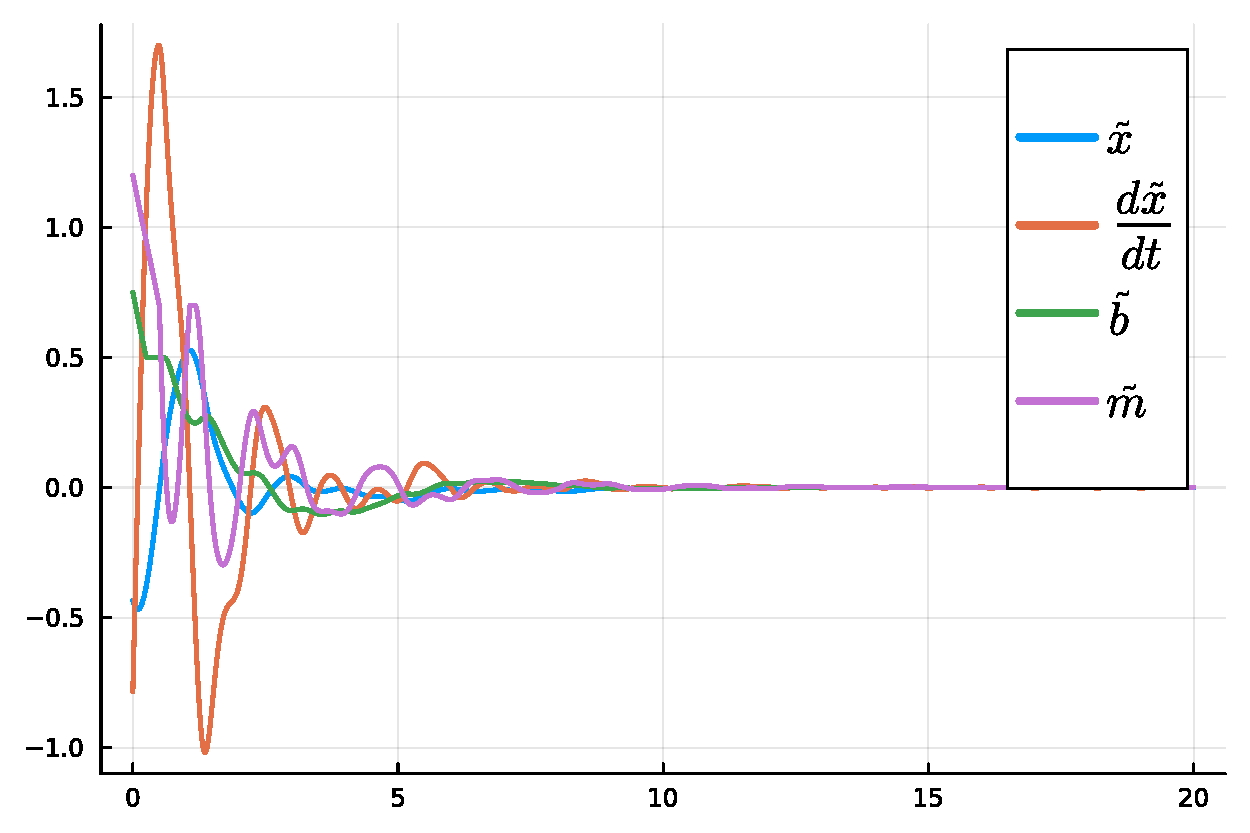
\includegraphics[width=0.5\textwidth]{./figures/adaptationrule2.pdf}
  \caption{Simulation showing that the system and estimation errors converge to
  zero.}
  \label{fig:adaptation}
\end{figure}

In Figure~\ref{fig:adaptation}, we plot the response of the system to the
control and adaptation laws~(\ref{eq:controller}, \ref{eq:adaptation}),
implemented in simulation. The constants that are used are as follows: $(A,
\omega, \varphi) = (\nicefrac{1}{2}, \pi, 60^\circ)$ and $(k, \lambda) = (1,
1)$. The real mass and damping of the system is $(m, b) = (0.7, 0.5)$ and their
estimates start at $(\hat{m}, \hat{b}) = (-\nicefrac{1}{2}, -\nicefrac{1}{4})$.

\begin{figure}[b]
  \centering
  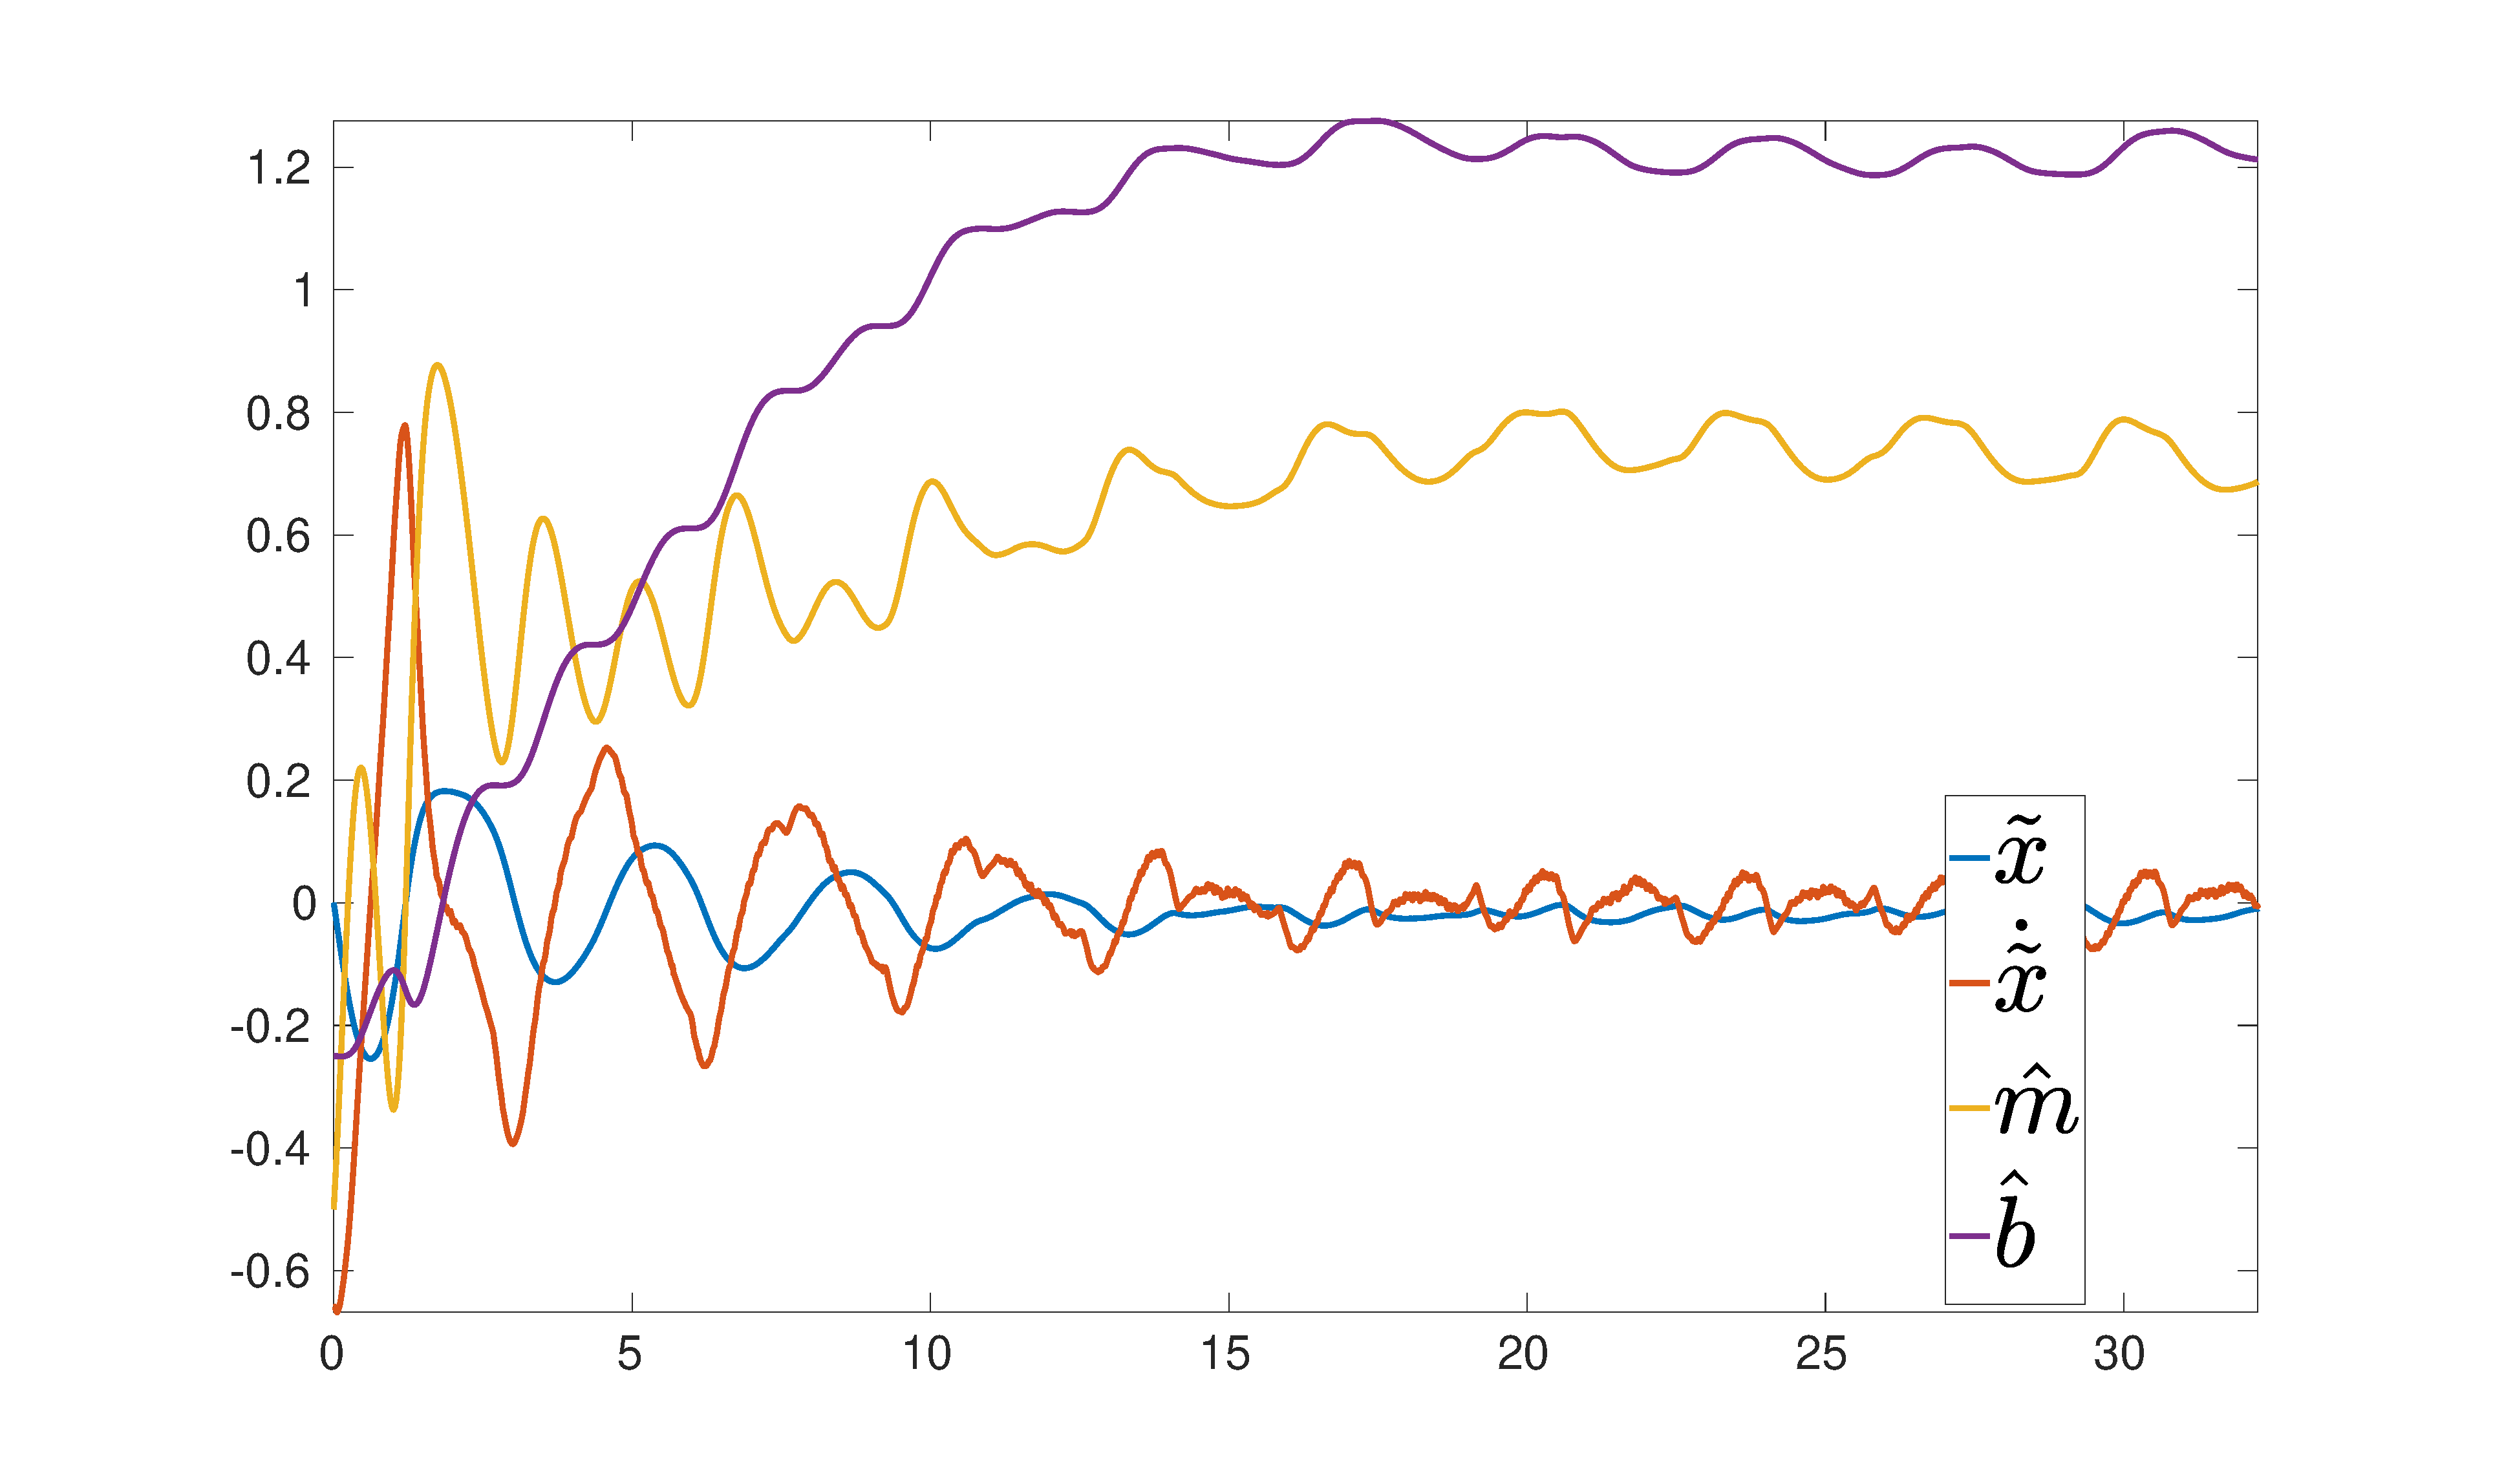
\includegraphics[width=0.5\textwidth]{./figures/station2_adaptation.eps}
  \caption{Hardware implementation of the estimation algorithm.}
  \label{fig:hardware}
\end{figure}

In Figure~\ref{fig:hardware}, we plot the response of the system to the control
and adaptation laws ~(\ref{eq:controller}, \ref{eq:adaptation}), implemented on
a real cart system. The constants used are as follows: $(A, \omega, \varphi) =
(\nicefrac{3}{10}, \nicefrac{3\pi}{5}, 0^\circ)$ and $(k, \lambda) = (1, 4)$. We
did not know the real mass and damping of the system and set our initial guesses
of them to be $(\hat{m}, \hat{b}) = (-\nicefrac{1}{2}, -\nicefrac{1}{4})$.

